\documentclass[a4paper, 12pt]{article}
\usepackage{lmodern}
\usepackage{amssymb,amsmath}
\usepackage{ifxetex,ifluatex}
\usepackage{fixltx2e} % provides \textsubscript
\ifnum 0\ifxetex 1\fi\ifluatex 1\fi=0 % if pdftex
  \usepackage[T1]{fontenc}
  \usepackage[utf8]{inputenc}
\else % if luatex or xelatex
  \ifxetex
    \usepackage{mathspec}
  \else
    \usepackage{fontspec}
  \fi
  \defaultfontfeatures{Ligatures=TeX,Scale=MatchLowercase}
\fi
% use upquote if available, for straight quotes in verbatim environments
\IfFileExists{upquote.sty}{\usepackage{upquote}}{}
% use microtype if available
\IfFileExists{microtype.sty}{%
\usepackage{microtype}
\UseMicrotypeSet[protrusion]{basicmath} % disable protrusion for tt fonts
}{}
\usepackage[left=3.5cm,right=2.5cm,top=2.5cm,bottom=2.5cm]{geometry}
\usepackage{hyperref}
\PassOptionsToPackage{usenames,dvipsnames}{color} % color is loaded by hyperref
\hypersetup{unicode=true,
            pdftitle={Redes Neurais e Regressão Polinomial},
            pdfauthor={Luiz Fernando Palin Droubi; Carlos Augusto Zilli; Norberto Hochheim},
            colorlinks=true,
            linkcolor=red,
            citecolor=green,
            urlcolor=magenta,
            breaklinks=true}
\urlstyle{same}  % don't use monospace font for urls
\usepackage{color}
\usepackage{fancyvrb}
\newcommand{\VerbBar}{|}
\newcommand{\VERB}{\Verb[commandchars=\\\{\}]}
\DefineVerbatimEnvironment{Highlighting}{Verbatim}{commandchars=\\\{\}}
% Add ',fontsize=\small' for more characters per line
\usepackage{framed}
\definecolor{shadecolor}{RGB}{248,248,248}
\newenvironment{Shaded}{\begin{snugshade}}{\end{snugshade}}
\newcommand{\KeywordTok}[1]{\textcolor[rgb]{0.13,0.29,0.53}{\textbf{#1}}}
\newcommand{\DataTypeTok}[1]{\textcolor[rgb]{0.13,0.29,0.53}{#1}}
\newcommand{\DecValTok}[1]{\textcolor[rgb]{0.00,0.00,0.81}{#1}}
\newcommand{\BaseNTok}[1]{\textcolor[rgb]{0.00,0.00,0.81}{#1}}
\newcommand{\FloatTok}[1]{\textcolor[rgb]{0.00,0.00,0.81}{#1}}
\newcommand{\ConstantTok}[1]{\textcolor[rgb]{0.00,0.00,0.00}{#1}}
\newcommand{\CharTok}[1]{\textcolor[rgb]{0.31,0.60,0.02}{#1}}
\newcommand{\SpecialCharTok}[1]{\textcolor[rgb]{0.00,0.00,0.00}{#1}}
\newcommand{\StringTok}[1]{\textcolor[rgb]{0.31,0.60,0.02}{#1}}
\newcommand{\VerbatimStringTok}[1]{\textcolor[rgb]{0.31,0.60,0.02}{#1}}
\newcommand{\SpecialStringTok}[1]{\textcolor[rgb]{0.31,0.60,0.02}{#1}}
\newcommand{\ImportTok}[1]{#1}
\newcommand{\CommentTok}[1]{\textcolor[rgb]{0.56,0.35,0.01}{\textit{#1}}}
\newcommand{\DocumentationTok}[1]{\textcolor[rgb]{0.56,0.35,0.01}{\textbf{\textit{#1}}}}
\newcommand{\AnnotationTok}[1]{\textcolor[rgb]{0.56,0.35,0.01}{\textbf{\textit{#1}}}}
\newcommand{\CommentVarTok}[1]{\textcolor[rgb]{0.56,0.35,0.01}{\textbf{\textit{#1}}}}
\newcommand{\OtherTok}[1]{\textcolor[rgb]{0.56,0.35,0.01}{#1}}
\newcommand{\FunctionTok}[1]{\textcolor[rgb]{0.00,0.00,0.00}{#1}}
\newcommand{\VariableTok}[1]{\textcolor[rgb]{0.00,0.00,0.00}{#1}}
\newcommand{\ControlFlowTok}[1]{\textcolor[rgb]{0.13,0.29,0.53}{\textbf{#1}}}
\newcommand{\OperatorTok}[1]{\textcolor[rgb]{0.81,0.36,0.00}{\textbf{#1}}}
\newcommand{\BuiltInTok}[1]{#1}
\newcommand{\ExtensionTok}[1]{#1}
\newcommand{\PreprocessorTok}[1]{\textcolor[rgb]{0.56,0.35,0.01}{\textit{#1}}}
\newcommand{\AttributeTok}[1]{\textcolor[rgb]{0.77,0.63,0.00}{#1}}
\newcommand{\RegionMarkerTok}[1]{#1}
\newcommand{\InformationTok}[1]{\textcolor[rgb]{0.56,0.35,0.01}{\textbf{\textit{#1}}}}
\newcommand{\WarningTok}[1]{\textcolor[rgb]{0.56,0.35,0.01}{\textbf{\textit{#1}}}}
\newcommand{\AlertTok}[1]{\textcolor[rgb]{0.94,0.16,0.16}{#1}}
\newcommand{\ErrorTok}[1]{\textcolor[rgb]{0.64,0.00,0.00}{\textbf{#1}}}
\newcommand{\NormalTok}[1]{#1}
\usepackage{graphicx,grffile}
\makeatletter
\def\maxwidth{\ifdim\Gin@nat@width>\linewidth\linewidth\else\Gin@nat@width\fi}
\def\maxheight{\ifdim\Gin@nat@height>\textheight\textheight\else\Gin@nat@height\fi}
\makeatother
% Scale images if necessary, so that they will not overflow the page
% margins by default, and it is still possible to overwrite the defaults
% using explicit options in \includegraphics[width, height, ...]{}
\setkeys{Gin}{width=\maxwidth,height=\maxheight,keepaspectratio}
\IfFileExists{parskip.sty}{%
\usepackage{parskip}
}{% else
\setlength{\parindent}{0pt}
\setlength{\parskip}{6pt plus 2pt minus 1pt}
}
\setlength{\emergencystretch}{3em}  % prevent overfull lines
\providecommand{\tightlist}{%
  \setlength{\itemsep}{0pt}\setlength{\parskip}{0pt}}
\setcounter{secnumdepth}{5}
% Redefines (sub)paragraphs to behave more like sections
\ifx\paragraph\undefined\else
\let\oldparagraph\paragraph
\renewcommand{\paragraph}[1]{\oldparagraph{#1}\mbox{}}
\fi
\ifx\subparagraph\undefined\else
\let\oldsubparagraph\subparagraph
\renewcommand{\subparagraph}[1]{\oldsubparagraph{#1}\mbox{}}
\fi

%%% Use protect on footnotes to avoid problems with footnotes in titles
\let\rmarkdownfootnote\footnote%
\def\footnote{\protect\rmarkdownfootnote}

%%% Change title format to be more compact
\usepackage{titling}

% Create subtitle command for use in maketitle
\newcommand{\subtitle}[1]{
  \posttitle{
    \begin{center}\large#1\end{center}
    }
}

\setlength{\droptitle}{-2em}

  \title{Redes Neurais e Regressão Polinomial}
    \pretitle{\vspace{\droptitle}\centering\huge}
  \posttitle{\par}
  \subtitle{Um estudo de caso}
  \author{Luiz Fernando Palin Droubi\footnote{UFSC,
  \href{mailto:luiz.droubi@planejamento.gov.br}{\nolinkurl{luiz.droubi@planejamento.gov.br}}} \\ Carlos Augusto Zilli\footnote{UFSC,
  \href{mailto:carloszilli@hotmail.com}{\nolinkurl{carloszilli@hotmail.com}}} \\ Norberto Hochheim\footnote{UFSC,
  \href{mailto:hochheim@gmail.com}{\nolinkurl{hochheim@gmail.com}}}}
    \preauthor{\centering\large\emph}
  \postauthor{\par}
      \predate{\centering\large\emph}
  \postdate{\par}
    \date{24/10/2018}

%\usepackage[brazil]{babel}
\usepackage{graphicx}
\usepackage{float}
\usepackage{subfig}
\usepackage{caption}
\usepackage{lastpage}
\setlength{\parindent}{1.25cm} % Default is 15pt.
\usepackage{indentfirst}
\usepackage{fontspec} % para Arial
\setmainfont{Arial}
\newcommand{\pkg}[1]{{\normalfont\fontseries{b}\selectfont #1}}
\let\proglang=\textsf
\let\code=\texttt
\usepackage{fancyhdr}
% Turn on the style
\pagestyle{fancy}
% Clear the header and footer
\fancyhead{}
\fancyfoot{}
% Set the right side of the footer to be the page number
\fancyfoot[R]{\thepage~/~\pageref{LastPage}}

\begin{document}
\maketitle

\begin{Shaded}
\begin{Highlighting}[]
\NormalTok{## Creating index variable }

\CommentTok{# Read the Data}
\NormalTok{data =}\StringTok{ }\NormalTok{centro_}\DecValTok{2015}\OperatorTok{@}\NormalTok{data[}\KeywordTok{complete.cases}\NormalTok{(centro_}\DecValTok{2015}\OperatorTok{@}\NormalTok{data),]}
\NormalTok{data}\OperatorTok{$}\NormalTok{padrao <-}\StringTok{ }\KeywordTok{as.numeric}\NormalTok{(data}\OperatorTok{$}\NormalTok{padrao)}

\CommentTok{# Random sampling}
\NormalTok{samplesize =}\StringTok{ }\FloatTok{0.60}\OperatorTok{*}\KeywordTok{nrow}\NormalTok{(data)}
\KeywordTok{set.seed}\NormalTok{(}\DecValTok{80}\NormalTok{)}
\NormalTok{index =}\StringTok{ }\KeywordTok{sample}\NormalTok{( }\KeywordTok{seq_len}\NormalTok{(}\KeywordTok{nrow}\NormalTok{(data)), }\DataTypeTok{size =}\NormalTok{ samplesize)}

\CommentTok{# Create training and test set}
\NormalTok{datatrain =}\StringTok{ }\NormalTok{data[ index, ]}
\NormalTok{datatest =}\StringTok{ }\NormalTok{data[ }\OperatorTok{-}\NormalTok{index, ]}
\end{Highlighting}
\end{Shaded}

\begin{Shaded}
\begin{Highlighting}[]
\NormalTok{## Scale data for neural network}
\NormalTok{max =}\StringTok{ }\KeywordTok{apply}\NormalTok{(data, }\DecValTok{2}\NormalTok{, max)}
\NormalTok{min =}\StringTok{ }\KeywordTok{apply}\NormalTok{(data, }\DecValTok{2}\NormalTok{, min)}
\NormalTok{scaled =}\StringTok{ }\KeywordTok{as.data.frame}\NormalTok{(}\KeywordTok{scale}\NormalTok{(data, }\DataTypeTok{center =}\NormalTok{ min, }\DataTypeTok{scale =}\NormalTok{ max }\OperatorTok{-}\StringTok{ }\NormalTok{min))}
\end{Highlighting}
\end{Shaded}

\begin{Shaded}
\begin{Highlighting}[]
\NormalTok{## Fit neural network }

\CommentTok{# creating training and test set}
\NormalTok{trainNN =}\StringTok{ }\NormalTok{scaled[index , ]}
\NormalTok{testNN =}\StringTok{ }\NormalTok{scaled[}\OperatorTok{-}\NormalTok{index , ]}

\CommentTok{# fit neural network}
\KeywordTok{set.seed}\NormalTok{(}\DecValTok{2}\NormalTok{)}
\NormalTok{NN =}\StringTok{ }\KeywordTok{neuralnet}\NormalTok{(valor }\OperatorTok{~}\StringTok{ }\NormalTok{area_total }\OperatorTok{+}\StringTok{ }\NormalTok{quartos }\OperatorTok{+}\StringTok{ }\NormalTok{suites }\OperatorTok{+}\StringTok{ }\NormalTok{garagens }\OperatorTok{+}\StringTok{ }
\StringTok{                 }\NormalTok{dist_b_mar }\OperatorTok{+}\StringTok{ }\NormalTok{padrao, }
               \DataTypeTok{data =}\NormalTok{ trainNN, }\DataTypeTok{hidden =} \DecValTok{2}\NormalTok{, }\DataTypeTok{linear.output =}\NormalTok{ T)}

\CommentTok{# plot neural network}
\KeywordTok{plot}\NormalTok{(NN)}
\end{Highlighting}
\end{Shaded}

\subsection{Estimativas}\label{estimativas}

\begin{Shaded}
\begin{Highlighting}[]
\NormalTok{## Prediction using neural network}

\NormalTok{predict_testNN =}\StringTok{ }\KeywordTok{compute}\NormalTok{(NN, testNN[,}\DecValTok{2}\OperatorTok{:}\DecValTok{7}\NormalTok{])}
\NormalTok{predict_testNN =}\StringTok{ }\NormalTok{(predict_testNN}\OperatorTok{$}\NormalTok{net.result }\OperatorTok{*}\StringTok{ }
\StringTok{                    }\NormalTok{(}\KeywordTok{max}\NormalTok{(data}\OperatorTok{$}\NormalTok{valor) }\OperatorTok{-}\StringTok{ }\KeywordTok{min}\NormalTok{(data}\OperatorTok{$}\NormalTok{valor))) }\OperatorTok{+}\StringTok{ }
\StringTok{                  }\KeywordTok{min}\NormalTok{(data}\OperatorTok{$}\NormalTok{valor)}

\KeywordTok{plot}\NormalTok{(datatest}\OperatorTok{$}\NormalTok{valor, predict_testNN, }\DataTypeTok{col=}\StringTok{'blue'}\NormalTok{, }\DataTypeTok{pch=}\DecValTok{16}\NormalTok{, }
     \DataTypeTok{ylab =} \StringTok{"predicted rating NN"}\NormalTok{, }\DataTypeTok{xlab =} \StringTok{"Valor"}\NormalTok{)}

\KeywordTok{abline}\NormalTok{(}\DecValTok{0}\NormalTok{,}\DecValTok{1}\NormalTok{)}
\end{Highlighting}
\end{Shaded}

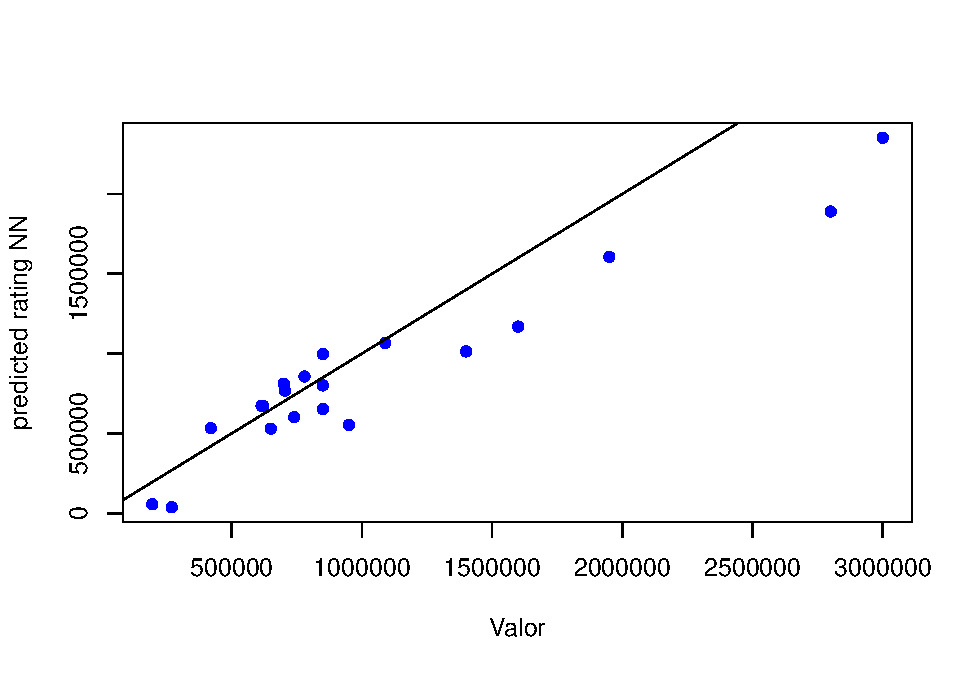
\includegraphics{Artigo_files/figure-latex/unnamed-chunk-4-1.pdf}

\begin{Shaded}
\begin{Highlighting}[]
\CommentTok{# Calculate Root Mean Square Error (RMSE)}
\NormalTok{RMSE.NN =}\StringTok{ }\NormalTok{(}\KeywordTok{sum}\NormalTok{((datatest}\OperatorTok{$}\NormalTok{valor }\OperatorTok{-}\StringTok{ }
\StringTok{                  }\NormalTok{predict_testNN)}\OperatorTok{^}\DecValTok{2}\NormalTok{) }\OperatorTok{/}\StringTok{ }\KeywordTok{nrow}\NormalTok{(datatest)) }\OperatorTok{^}\StringTok{ }\FloatTok{0.5}
\end{Highlighting}
\end{Shaded}

\subsection{Validação Cruzada}\label{validacao-cruzada}

\begin{Shaded}
\begin{Highlighting}[]
\NormalTok{## Cross validation of neural network model}

\CommentTok{# Load libraries}
\KeywordTok{library}\NormalTok{(boot)}
\KeywordTok{library}\NormalTok{(plyr)}

\CommentTok{# Initialize variables}
\KeywordTok{set.seed}\NormalTok{(}\DecValTok{50}\NormalTok{)}
\NormalTok{k =}\StringTok{ }\DecValTok{100}
\NormalTok{RMSE.NN =}\StringTok{ }\OtherTok{NULL}
\NormalTok{n <-}\StringTok{ }\KeywordTok{nrow}\NormalTok{(data)}

\NormalTok{List =}\StringTok{ }\KeywordTok{list}\NormalTok{()}

\CommentTok{# Fit neural network model within nested for loop}
\ControlFlowTok{for}\NormalTok{(j }\ControlFlowTok{in} \KeywordTok{seq}\NormalTok{(}\FloatTok{0.2}\NormalTok{, }\FloatTok{0.9}\NormalTok{, }\FloatTok{0.02}\NormalTok{))\{}
    \ControlFlowTok{for}\NormalTok{ (i }\ControlFlowTok{in} \DecValTok{1}\OperatorTok{:}\NormalTok{k) \{}
\NormalTok{        index =}\StringTok{ }\KeywordTok{sample}\NormalTok{(}\DecValTok{1}\OperatorTok{:}\NormalTok{n,j}\OperatorTok{*}\NormalTok{n )}

\NormalTok{        trainNN =}\StringTok{ }\NormalTok{scaled[index,]}
\NormalTok{        testNN =}\StringTok{ }\NormalTok{scaled[}\OperatorTok{-}\NormalTok{index,]}
\NormalTok{        datatest =}\StringTok{ }\NormalTok{data[}\OperatorTok{-}\NormalTok{index,]}

\NormalTok{        NN =}\StringTok{ }\KeywordTok{neuralnet}\NormalTok{(valor }\OperatorTok{~}\StringTok{ }\NormalTok{area_total }\OperatorTok{+}\StringTok{ }\NormalTok{quartos }\OperatorTok{+}\StringTok{ }\NormalTok{suites }\OperatorTok{+}\StringTok{ }
\StringTok{                         }\NormalTok{garagens }\OperatorTok{+}\StringTok{ }\NormalTok{dist_b_mar }\OperatorTok{+}\StringTok{ }\NormalTok{padrao,}
\NormalTok{                       trainNN, }\DataTypeTok{hidden =} \DecValTok{1}\NormalTok{, }\DataTypeTok{linear.output=}\NormalTok{ T)}
\NormalTok{        predict_testNN =}\StringTok{ }\KeywordTok{compute}\NormalTok{(NN,testNN[,}\KeywordTok{c}\NormalTok{(}\DecValTok{2}\OperatorTok{:}\DecValTok{7}\NormalTok{)])}
\NormalTok{        predict_testNN =}\StringTok{ }\NormalTok{(predict_testNN}\OperatorTok{$}\NormalTok{net.result}\OperatorTok{*}
\StringTok{                            }\NormalTok{(}\KeywordTok{max}\NormalTok{(data}\OperatorTok{$}\NormalTok{valor) }\OperatorTok{-}\StringTok{ }\KeywordTok{min}\NormalTok{(data}\OperatorTok{$}\NormalTok{valor))) }\OperatorTok{+}
\StringTok{                          }\KeywordTok{min}\NormalTok{(data}\OperatorTok{$}\NormalTok{valor)}

\NormalTok{        RMSE.NN[i]<-}\StringTok{ }\KeywordTok{sqrt}\NormalTok{(}\KeywordTok{sum}\NormalTok{((datatest}\OperatorTok{$}\NormalTok{valor }\OperatorTok{-}\StringTok{ }\NormalTok{predict_testNN)}\OperatorTok{^}\DecValTok{2}\NormalTok{)}\OperatorTok{/}
\StringTok{                            }\KeywordTok{nrow}\NormalTok{(datatest))}
\NormalTok{    \}}
\NormalTok{    List[[j}\OperatorTok{*}\NormalTok{n]] =}\StringTok{ }\NormalTok{RMSE.NN}
\NormalTok{\}}

\NormalTok{Matrix.RMSE =}\StringTok{ }\KeywordTok{do.call}\NormalTok{(cbind, List)}

\NormalTok{## Prepare boxplot}
\KeywordTok{boxplot}\NormalTok{(Matrix.RMSE[,}\DecValTok{36}\NormalTok{], }
        \DataTypeTok{ylab =} \StringTok{"RMSE"}\NormalTok{, }
        \DataTypeTok{main =} \StringTok{"RMSE BoxPlot (length of traning set = 45)"}\NormalTok{)}
\end{Highlighting}
\end{Shaded}

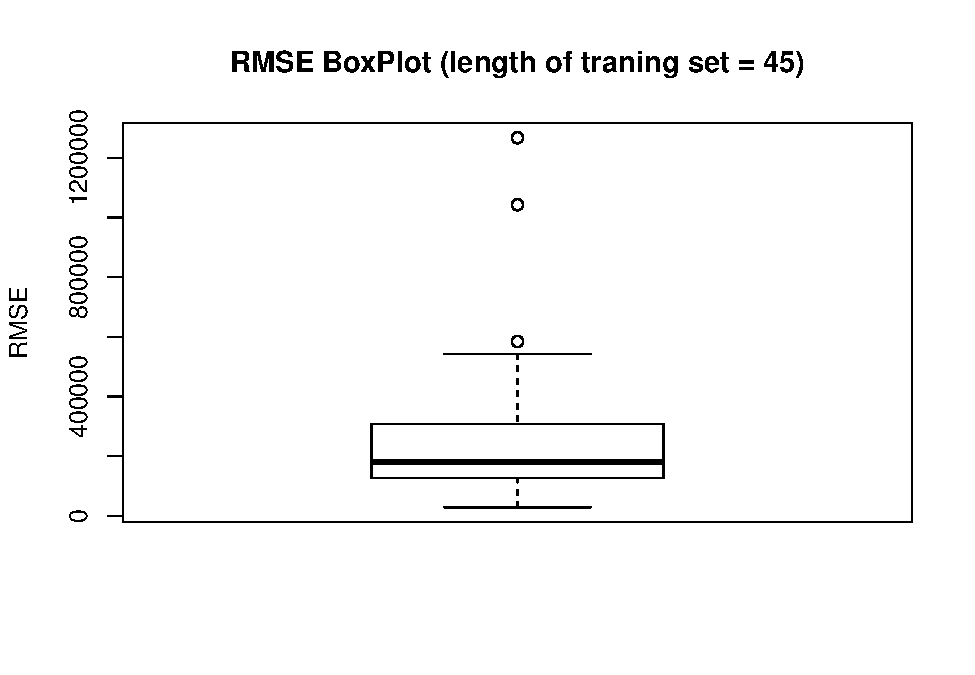
\includegraphics{Artigo_files/figure-latex/unnamed-chunk-5-1.pdf}

\begin{Shaded}
\begin{Highlighting}[]
\NormalTok{## Variation of median RMSE }
\KeywordTok{library}\NormalTok{(matrixStats)}

\NormalTok{med =}\StringTok{ }\KeywordTok{colMedians}\NormalTok{(Matrix.RMSE)}

\NormalTok{X =}\StringTok{ }\KeywordTok{seq}\NormalTok{(}\FloatTok{0.2}\NormalTok{, }\FloatTok{0.9}\NormalTok{, }\FloatTok{0.02}\NormalTok{)}\OperatorTok{*}\NormalTok{n}

\KeywordTok{plot}\NormalTok{ (med}\OperatorTok{~}\NormalTok{X, }\DataTypeTok{type =} \StringTok{"l"}\NormalTok{, }
      \DataTypeTok{xlab =} \StringTok{"length of training set"}\NormalTok{, }
      \DataTypeTok{ylab =} \StringTok{"median RMSE"}\NormalTok{, }
      \DataTypeTok{main =} \StringTok{"Variation of RMSE with length of training set"}\NormalTok{)}
\end{Highlighting}
\end{Shaded}

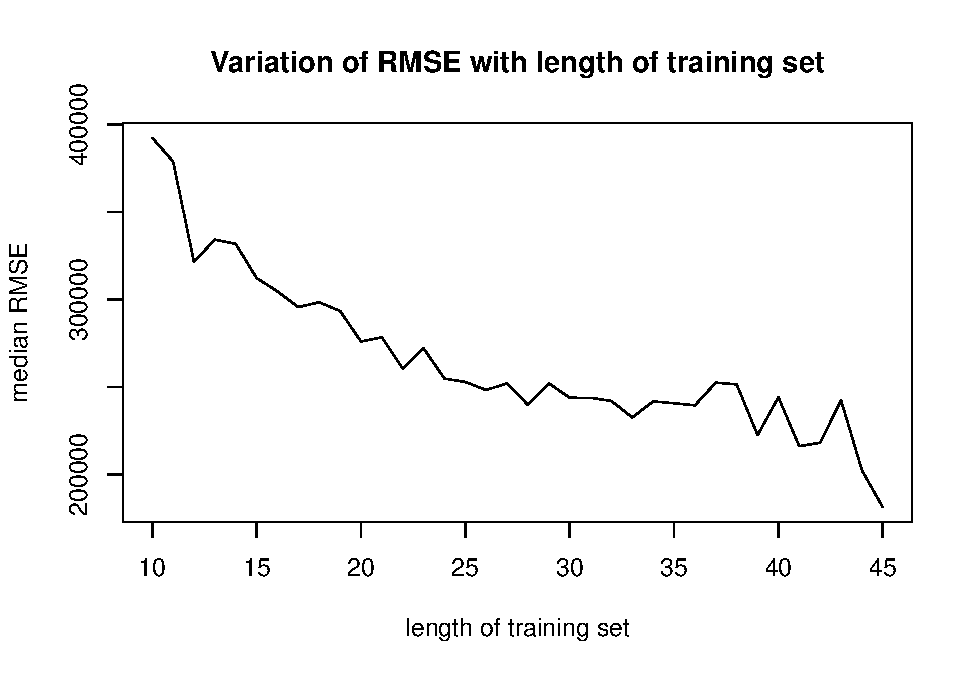
\includegraphics{Artigo_files/figure-latex/unnamed-chunk-6-1.pdf}

\section{REGRESSÃO POLINOMIAL}\label{regressao-polinomial}

\begin{Shaded}
\begin{Highlighting}[]
\NormalTok{data <-}\StringTok{ }\KeywordTok{cbind}\NormalTok{(data[, }\OperatorTok{-}\DecValTok{1}\NormalTok{], data[,}\DecValTok{1}\NormalTok{])}

\CommentTok{# Initialize variables}
\KeywordTok{set.seed}\NormalTok{(}\DecValTok{50}\NormalTok{)}
\NormalTok{k =}\StringTok{ }\DecValTok{100}
\NormalTok{RMSE.PR =}\StringTok{ }\OtherTok{NULL}
\NormalTok{n <-}\StringTok{ }\KeywordTok{nrow}\NormalTok{(data)}

\NormalTok{List =}\StringTok{ }\KeywordTok{list}\NormalTok{()}

\CommentTok{# Fit PR model within nested for loop}
\ControlFlowTok{for}\NormalTok{(j }\ControlFlowTok{in} \KeywordTok{seq}\NormalTok{(}\FloatTok{0.2}\NormalTok{, }\FloatTok{0.9}\NormalTok{, }\FloatTok{0.02}\NormalTok{))\{}
  \ControlFlowTok{for}\NormalTok{ (i }\ControlFlowTok{in} \DecValTok{1}\OperatorTok{:}\NormalTok{k) \{}
\NormalTok{    index =}\StringTok{ }\KeywordTok{sample}\NormalTok{(}\DecValTok{1}\OperatorTok{:}\NormalTok{n,j}\OperatorTok{*}\NormalTok{n )}
\NormalTok{    trainPR =}\StringTok{ }\NormalTok{data[index,]}
\NormalTok{    testPR =}\StringTok{ }\NormalTok{data[}\OperatorTok{-}\NormalTok{index,]}
\NormalTok{    polyFit.out <-}\StringTok{ }\KeywordTok{polyFit}\NormalTok{(trainPR, }\DataTypeTok{deg =} \DecValTok{2}\NormalTok{, }\DataTypeTok{maxInteractDeg =} \DecValTok{2}\NormalTok{, }
                           \DataTypeTok{use =} \StringTok{"lm"}\NormalTok{, }\DataTypeTok{pcaMethod =} \StringTok{"prcomp"}\NormalTok{)}
\NormalTok{    predict_testPR =}\StringTok{ }\KeywordTok{predict}\NormalTok{(polyFit.out, testPR[,}\KeywordTok{c}\NormalTok{(}\DecValTok{1}\OperatorTok{:}\DecValTok{6}\NormalTok{)])}
\NormalTok{    RMSE.PR[i]<-}\StringTok{ }\KeywordTok{sqrt}\NormalTok{(}\KeywordTok{sum}\NormalTok{((testPR}\OperatorTok{$}\NormalTok{valor }\OperatorTok{-}\StringTok{ }\NormalTok{predict_testPR)}\OperatorTok{^}\DecValTok{2}\NormalTok{)}\OperatorTok{/}
\StringTok{                        }\KeywordTok{nrow}\NormalTok{(trainPR))}
\NormalTok{    \}}
\NormalTok{  List[[j}\OperatorTok{*}\NormalTok{n]] =}\StringTok{ }\NormalTok{RMSE.PR}
\NormalTok{\}}


\NormalTok{Matrix.RMSE =}\StringTok{ }\KeywordTok{do.call}\NormalTok{(cbind, List)}

\NormalTok{## Prepare boxplot}
\KeywordTok{boxplot}\NormalTok{(Matrix.RMSE[,}\DecValTok{36}\NormalTok{], }
        \DataTypeTok{ylab =} \StringTok{"RMSE"}\NormalTok{, }
        \DataTypeTok{main =} \StringTok{"RMSE BoxPlot (length of traning set = 45)"}\NormalTok{)}
\end{Highlighting}
\end{Shaded}

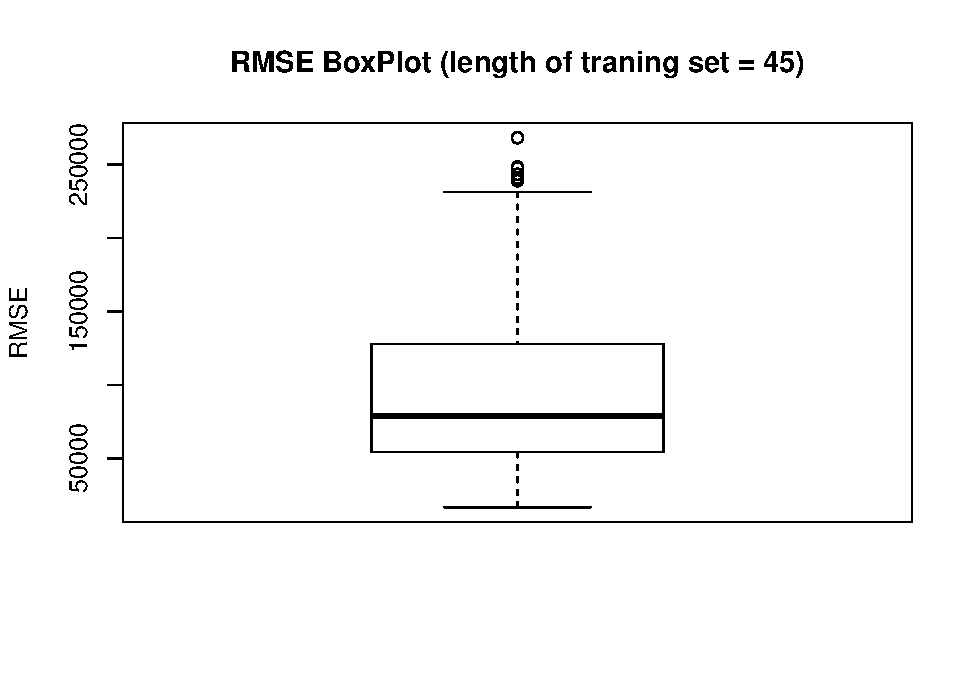
\includegraphics{Artigo_files/figure-latex/unnamed-chunk-7-1.pdf}

\begin{Shaded}
\begin{Highlighting}[]
\NormalTok{## Variation of median RMSE }
\NormalTok{med =}\StringTok{ }\KeywordTok{colMedians}\NormalTok{(Matrix.RMSE)}

\NormalTok{X =}\StringTok{ }\KeywordTok{seq}\NormalTok{(}\FloatTok{0.2}\NormalTok{, }\FloatTok{0.9}\NormalTok{, }\FloatTok{0.02}\NormalTok{)}\OperatorTok{*}\NormalTok{n}

\KeywordTok{plot}\NormalTok{ (med}\OperatorTok{~}\NormalTok{X, }\DataTypeTok{type =} \StringTok{"l"}\NormalTok{, }
      \DataTypeTok{xlab =} \StringTok{"length of training set"}\NormalTok{, }
      \DataTypeTok{ylab =} \StringTok{"median RMSE"}\NormalTok{, }
      \DataTypeTok{main =} \StringTok{"Variation of RMSE with length of training set"}\NormalTok{)}
\end{Highlighting}
\end{Shaded}

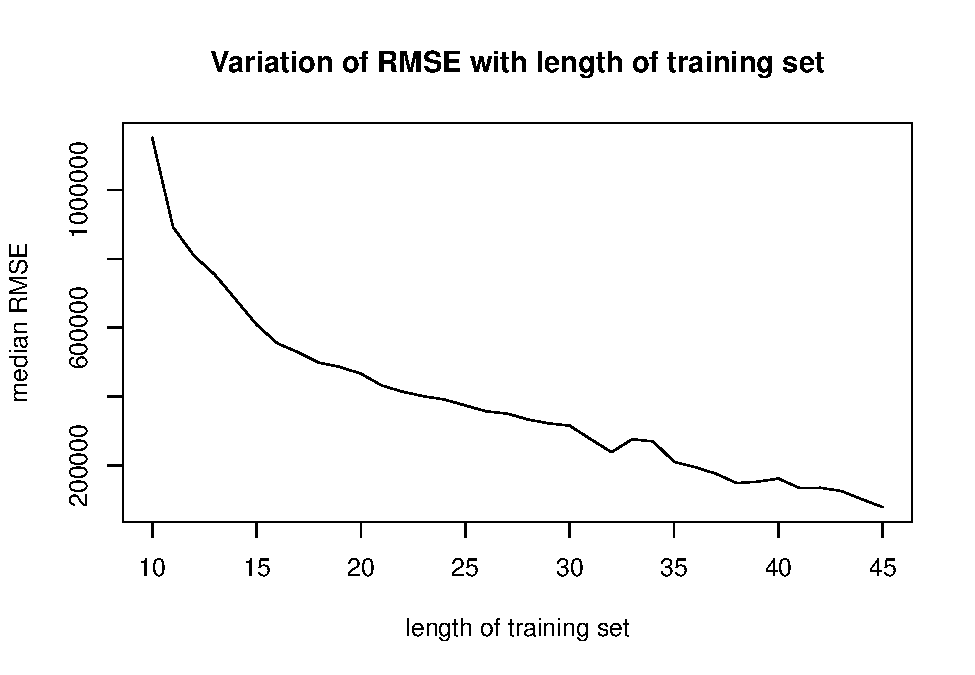
\includegraphics{Artigo_files/figure-latex/unnamed-chunk-8-1.pdf}

\section{CONCLUSÕES E RECOMENDAÇÕES}\label{conclusoes-e-recomendacoes}

\section{REFERÊNCIAS}\label{referencias}


\end{document}
